\documentclass[11pt]{article}
\usepackage{enumerate}
\usepackage{fancyhdr}
\usepackage{amsmath}
\usepackage{graphicx}

\thispagestyle{empty}
\setlength{\parindent}{0cm}
\setlength{\parskip}{0.3cm plus4mm minus3mm}
\oddsidemargin = 0.0in
\textwidth = 6.5 in
\textheight = 9 in
\headsep = 0in

\title{CSCI 4100 Fall 2018 \\
% enter assignment number
Assignment 7 Answers}
\author{Damin Xu\\661679187}



\begin{document}
\maketitle
% enter question #
\noindent{\bf Classifying Handwritten Digits: 1 vs. 5}
\begin{enumerate} [(a)]
	\item \ \\
	\begin{figure}[htbp]
		\centering
		\begin{minipage}[t]{0.48\textwidth}
			\centering
			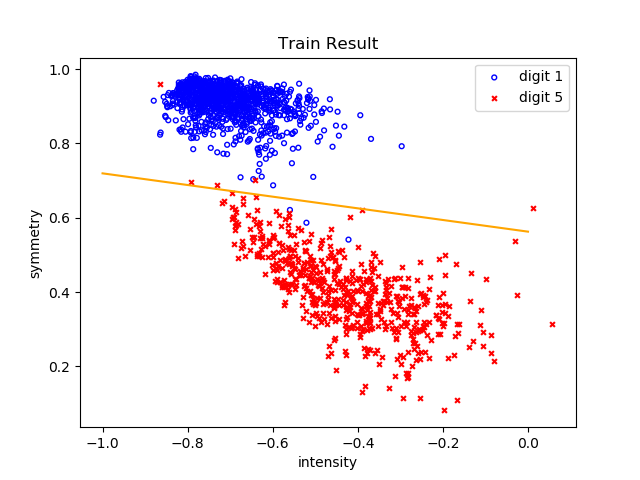
\includegraphics[width=8.5cm]{train_result.png}
		\end{minipage}
		\begin{minipage}[t]{0.48\textwidth}
			\centering
			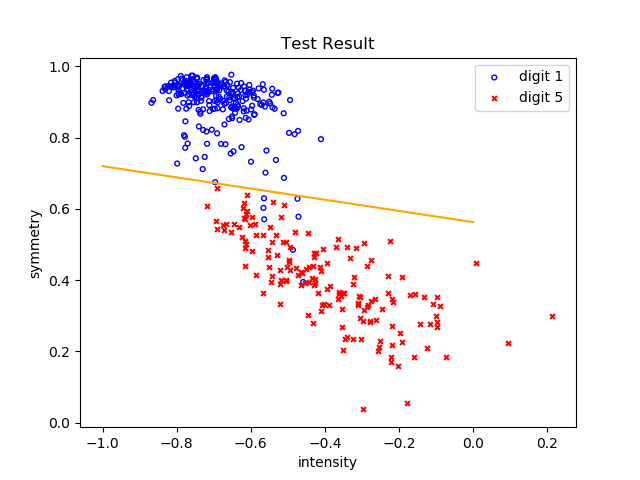
\includegraphics[width=8.5cm]{test_result.png}
		\end{minipage}
	\end{figure}

	\item $E_{in} = 0.00512 = 0.512\%$\\$E_{test} = 0.0165=1.65\%$

	\item Bound based on $E_{in} = 0.0594$\\
	Bound based on $E_{test} = 0.114$
	\newpage
	\item \
	\begin{figure}[htbp]
		\centering
		\begin{minipage}[t]{0.48\textwidth}
			\centering
			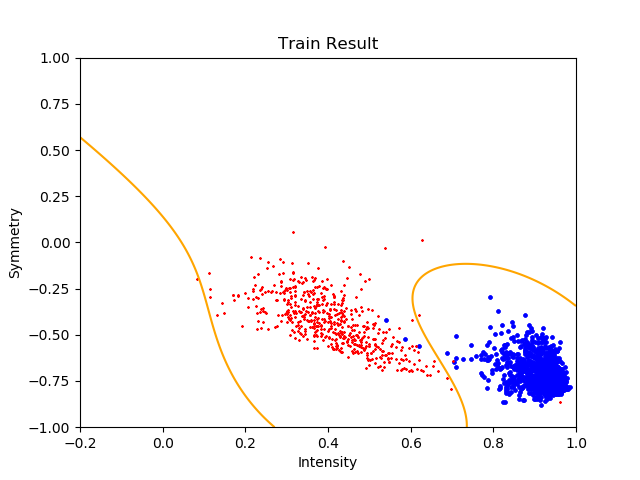
\includegraphics[width=8.5cm]{train_result1.png}
		\end{minipage}
		\begin{minipage}[t]{0.48\textwidth}
			\centering
			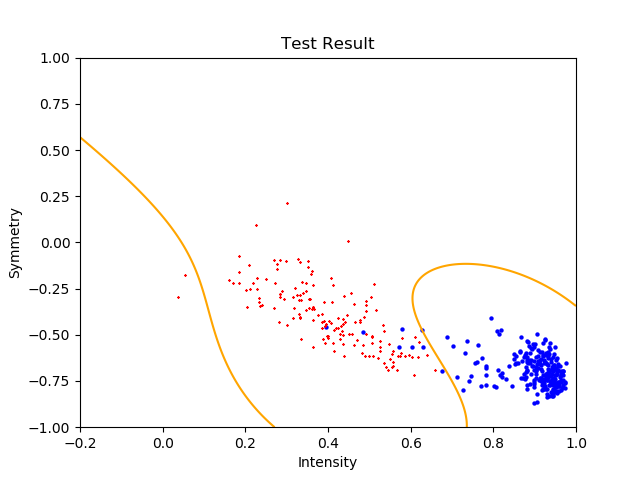
\includegraphics[width=8.5cm]{test_result1.png}
		\end{minipage}
	\end{figure}
	$E_{in} = 0.00448 = 0.448\%$\\$E_{test} = 0.0212=2.12\%$\\
	Bound based on $E_{in} = 0.0601$\\
	Bound based on $E_{test} = 0.115$

	\item I will choose the linear model without the $3^{rd}$ order polynomial transform linear, because the linear transformation will cause overfitting which leads to a larger $E_{out}$
\end{enumerate}
\newpage

\noindent{\bf Gradient Descent on a “Simple” Function}
\begin{enumerate} [(a)]
	\item The left one is when learning rate = 0.01 and the right one is when learning rate = 0.1 
		\begin{figure}[htbp]
		\centering
		\begin{minipage}[t]{0.48\textwidth}
			\centering
			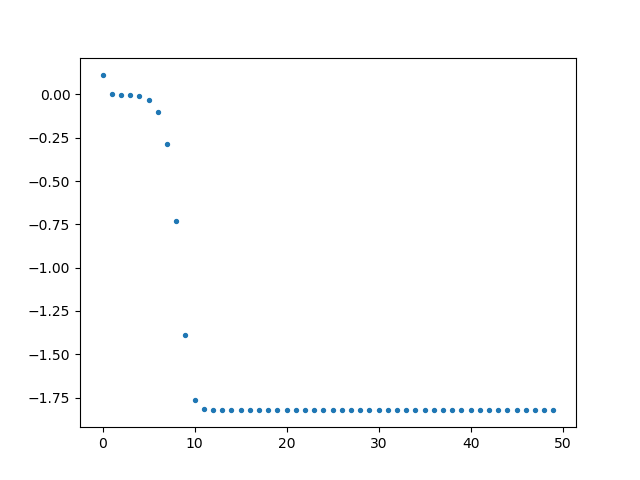
\includegraphics[width=8.5cm]{2_1.png}
		\end{minipage}
		\begin{minipage}[t]{0.48\textwidth}
			\centering
			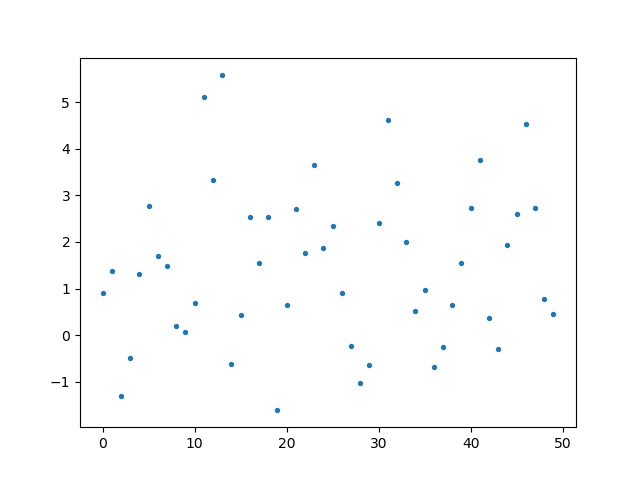
\includegraphics[width=8.5cm]{2_2.png}
		\end{minipage}
	\end{figure}
	When learning rate = 0.1, the value of function jumps up and down.

	\item \ \\
	\begin{tabular}{|l|l|l|l|}
	\hline
	          & x                  & y                  & f(x,y)            \\
	(0.1,0.1) & 0.243804968878158  & -0.237925821319047 & -1.82007854154716 \\
	(1,1)     & 1.21807030090520   & 0.712811950338754  & 0.593269374325836 \\
	(0.5,0.5) & -0.731377459870107 & -0.237855362955527 & -1.33248106233098 \\
	(-1,-1)   & -1.21807030090520  & -0.712811950338754 & 0.593269374325836
	\end{tabular}
\end{enumerate}

\newpage

\noindent{\bf Problem 3.16}
\begin{enumerate} [(a)]
	\item $cost(accept)=P[y=1|x]\times 0 +P[y=-1|x]\times c_a = (1-g(x))c_a$\\$cost(reject)=P[y=1|x]\times c_a +P[y=-1|x]\times 0 =  g(x)c_a$

	\item Here we only want $cost(accept)\leq cost(reject)$, so\[
		(1-g(x))c_a \leq g(x)c_a
	\]\[
		c_a-g(x)c_a \leq g(x)c_a
	\]\[
		c_a \leq g(x)(c_a+c_r)
	\]\[
		g(x) \geq \frac{c_a}{c_a+c_r}
	\]
	Therefore, when $g(x) \geq \frac{c_a}{c_a+c_r}$, we will accept, so $k= \frac{c_a}{c_a+c_r}$

	\item \[
		k_{supermarket} = \frac{1}{1+10}=\frac{1}{11}
	\]\[
		l_{CIA} = \frac{1000}{1000+1} = \frac{1000}{1001}
	\]
	CIA accept the fingerprint only when g(x) is large.
\end{enumerate}

\end{document}
\end{document}
